%
% GNU courseware, XIN YUAN, 2017
%

\section{遗传算法}\fontsize{10pt}{10pt}\selectfont

\frame{\frametitle{遗传算法}
	\begin{itemize}
		\item<1-> 遗传算法概述
		\item<2-> 遗传算法原理
		\item<3-> 遗传算法应用
	\end{itemize}
}

\frame{\frametitle{遗传算法概述}
\ \ \ \ 遗传算法模拟自然选择和自然遗传过程中发生的繁\\
殖、交叉和基因突变现象,在每次迭代中都保留一组候\\
选解,并按某种指标从解群中选取较优的个体,利用遗\\
传算子(选择、交叉和变异)对这些个体进行组合,产生\\
新一代的候选解群,重复此过程,直到满足某种收敛指\\标为止。
}


\frame{\frametitle{基本遗传算法}
\ \ \ \ \ \ 基本遗传算法(Simple Genetic Algorithms,\\
简称SGA,又称简单遗传算法或标准遗传算法),\\
是由Goldberg总结出的一种最基本的遗传算法,\\
其遗传进化操作过程简单,容易理解,是其它一\\
些遗传算法的雏形和基础。 
}


\frame{\frametitle{遗传算法过程}
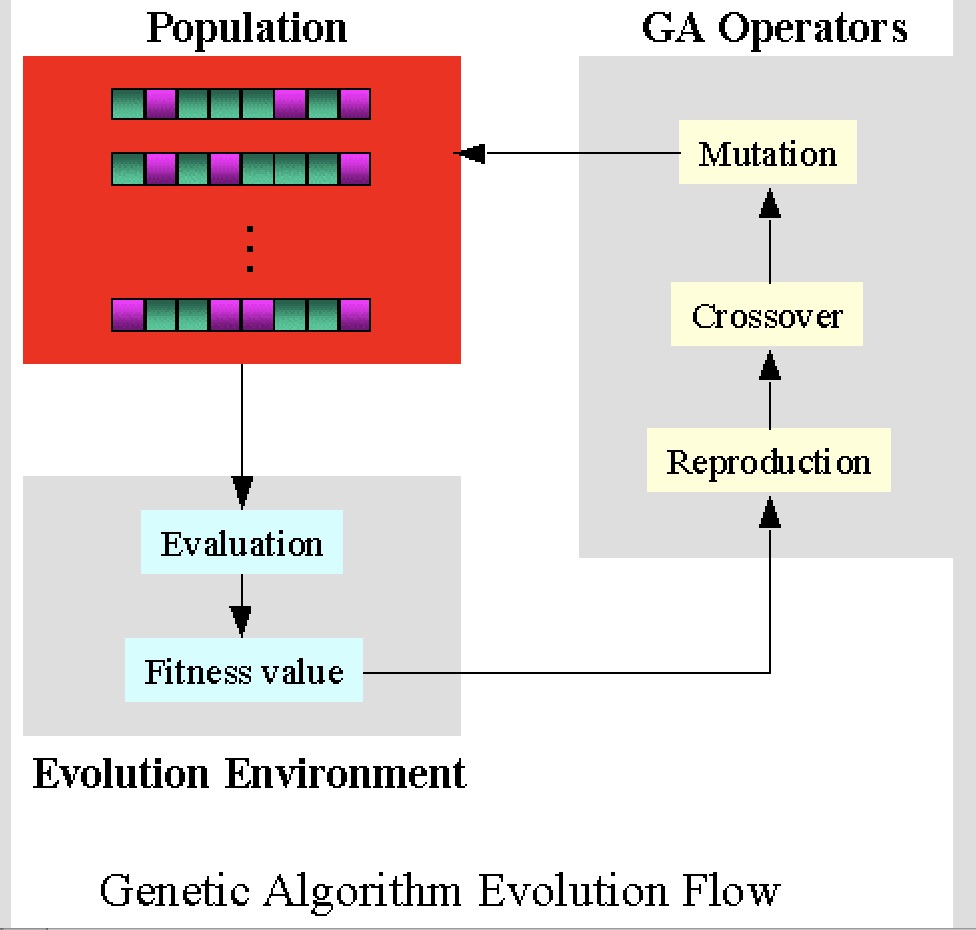
\includegraphics[width=0.8\textwidth]{evolutionflow.jpg}
}

\frame{\frametitle{基本遗传算法的组成}
(1)编码:通过某种编码机制把对象抽象
为由特定符号按一定顺序排成的串。
SGA使用二进制串进行编码。 \\
(2)适应度函数:遗传算法对一个个体(解)
的好坏用适应度函数值来评价,适应度函数值越大,解的质量越好。\\

}

\frame{\frametitle{基本遗传算法的组成}
(3)遗传算子(选择、交叉、变异)\\
选择算子:优胜劣汰操作,适应度高的个体被遗传到下一代群体中的概率大;
适应度低的个体,被遗传到下一代群体中的概率小。SGA中选择算子采用轮盘
赌选择方法。\\
交叉:对两个相互配对的染色体依据交叉概率 Pc 按某种方式相互交换其部分
基因,从而形成两个新的个体。SGA中交叉算子采用单点交叉算子。\\
变异算子: 依据变异概率 Pm 将个体编码串中的某些基因值用其它基因
值来替换,从而形成一个新的个体 。SGA中变异算子采用基本位变异算子。\\
}

\frame{\frametitle{基本遗传算法的组成}
(4)运行参数\\
M  : 种群规模 \\
T  : 遗传运算的终止进化代数 \\
Pc  : 交叉概率 \\
Pm : 变异概率 \\
}

\frame{\frametitle{遗传算法原理}
模式定理:具有低阶、短定义距以及平均适应度高于种群平均适应度的模式在子代中呈指数增长。\\

积木块假设:遗传算法通过短定义距、低阶以及高平均适应度的模式(积木块),在遗传操作下相互
结合,最终接近全局最优解。\\

模式定理保证了较优模式的样本数呈指数增长,从而使遗传算法找到全局最优解的可能性存在;\\
而积木块假设则指出了在遗传算子的作用下,能生成全局最优解。 \\

}

\frame{\frametitle{遗传算法应用}
(1)组合优化     (2)函数优化\\ 
(3)自动控制     (4)生产调度\\
(5)图像处理      (6)机器学习\\
(7)人工生命      (8)数据挖掘\\
}

%end
